% TeX encoding = utf8
% TeX spellcheck = pl_PL 
\documentclass[a4paper, 12pt]{article}
\usepackage[utf8]{inputenc}
\usepackage[polish]{babel}
\usepackage{polski}
\usepackage{float}
\usepackage{graphicx}
\usepackage{listings}
\usepackage{amsfonts}
\usepackage{geometry}
\usepackage{multicol}
\usepackage{latexsym}
\usepackage{enumerate}
\usepackage{hyperref}
\usepackage{wrapfig}
\usepackage{color} %red, green, blue, yellow, cyan, magenta, black, white
\definecolor{mygreen}{RGB}{28,172,0} % color values Red, Green, Blue
\definecolor{mylilas}{RGB}{170,55,241}

 \renewcommand{\familydefault}{\sfdefault}


\author{Marcin Dziedzic}
\title{[MNUM] - Dokumentacja projektu  nr 4}
\frenchspacing

\newgeometry{tmargin=2cm, bmargin=2cm, lmargin=2cm, rmargin=2cm}
\pagestyle{empty}


\begin{document}

\lstset{language=Matlab,%
    basicstyle=\color{red},
    breaklines=true,%
    morekeywords={matlab2tikz},
    keywordstyle=\color{blue},%
    morekeywords=[2]{1}, keywordstyle=[2]{\color{black}},
    identifierstyle=\color{black},%
    stringstyle=\color{mylilas},%
    commentstyle=\color{mygreen},%
    showstringspaces=false,
    numbers=right,%
    numberstyle={ \color{black}},% size of the numbers
    numbersep=5pt, % this defines how far the numbers are from the text
    emph=[1]{for,endfor,endwhile,endfunction,endif,break},emphstyle=[1]\color{blue}, %some words to emphasise
    emph=[2]{,.}, emphstyle=[2]\color{yellow},%
}

\maketitle

\section{Zadanie 1}
\subsection{Polecenie}
Ruch punktu jest opisany równaniami:
$$ x_{1}' = x_{2} + x_{1}(0,2 - x_{1}^{2} - x_{2}^{2}) $$
$$ x_{2}' = -x_{1} + x_{2}(0,2 - x_{1}^{2} - x_{2}^{2}) $$\\
Należy obliczyć przebieg trajektorii na przedziale [0.20] dla następujących warunków początkowych: \\
\\
 $$a) x_{1}(0) = 8 ,  x_{2}(0) = 7 $$
 $$b) x_{1}(0) = 0 , x_{2}(0) = 0,4 $$
 $$c) x_{1}(0) = 5 , x_{2}(0) = 0 $$
 $$d) x_{1}(0) = 0,01 , x_{2}(0) = 0,001 $$
 
\subsection{Ogólny opis zagadnienia rozwiązywania układu równań różniczkowych}
Rozważane jest zagadnienie układu równań (pogrubione wartości to wektory) różniczkowych zwyczajnych pierwszego rzędu (ale mogą być one nieliniowe).
Dane jest równanie (układ rówań):\\
$ \mathbf{x'}(t) = \mathbf{f}(t,\mathbf{x}) $, przy czym \textbf{x} to szukana funkcja. Znany jest przedział, na którym szukamy \textbf{x}: $t \in [a,b]$ oraz warunki początkowe: $\mathbf{x}(a)$, .Wyróżnia się metody jednokrokowe, bazujące tylko na punckie otzymanym w poprzedniej iteracji, oraz metody wielokrokowe, które opierają się na większej liczbie punktów.\\

\section{Metoda RK4 ze stałym krokiem}

\subsection{Opis algorytmu}
Metody Rungego - Kutty to grupa metod jednokrokowych. Na przedziale $[t_{n}, t_{n} + h]$ obliczane są pochodne \textbf{x} (poprzez podstawienie do funkcji \textbf{f} danej równaniu), w różnych punktach w badanym przedziale, a następnie badana funkcja jest przybliżana przez pewną liniową kombinację tych pochodnych. Kompromisem pomiędzy dokładnością (rzędem metody) a nakładem obliczeń na jedną iterację jest metoda RK4 (obliczenie pochodnej w 4 punktach). Wzory opisujące jedną iterację:
$$ \mathbf{x_{n+1}} = \mathbf{x_{n}} + \frac{1}{6}h(\mathbf{k_{1}} + 2\mathbf{k_{2}} + 2\mathbf{k_{3}} + \mathbf{k_{4}})$$
$$\mathbf{k_{1}} = \mathbf{f}(t_{n}, \mathbf{x_{n}})$$
$$\mathbf{k_{2}} = \mathbf{f}(t_{n}+\frac{1}{2}h, \mathbf{x_{n}} + \frac{1}{2}h\mathbf{k_{1}})$$
$$\mathbf{k_{3}} = \mathbf{f}(t_{n}+\frac{1}{2}h, \mathbf{x_{n}} + \frac{1}{2}h\mathbf{k_{2}})$$
$$\mathbf{k_{4}} = \mathbf{f}(t_{n}+h, \mathbf{x_{n}} + h\mathbf{k_{3}}$$\\



\subsection{Kod funkcji zwracającej punkt określony równaniami}
\begin{lstlisting}
function [D] = md_fx(x)
% Funkcja zwracajaca pochodne  
D(1) = x(2) + x(1)*(0.2 -x(1)^2 -x(2)^2); 
D(2) = -x(1) + x(2)*(0.2 -x(1)^2 -x(2)^2);
end
\end{lstlisting}
\hspace{5cm}
\subsection{Kod funkcji zwracającej rozwiązania metodą RK4}
\begin{lstlisting}
function [Y] = md_rk4s(x,timelimit,stp)
% Rozwiazanie ukladu metoda Rungego-Kutty czwartego rzedu
% x - stan poczatkowy
% timelimit - zakres czasu
% step - rozmiar kroku

    Y = zeros(ceil(timelimit/stp),3); %macierz stanow x1, x2 i czasu
    hstp=stp/2; %polowa kroku
    for i = 1:(ceil(timelimit/stp))
        Y(i,3) = i*stp;  
        k1 = md_fx(x); 
        k2 = md_fx(x+hstp*k1); 
        k3 = md_fx(x+hstp*k2); 
        k4 = md_fx(x+stp*k3); 
        x=x+(1/6)*stp*(k1+2*k2+2*k3+k4); 
        Y(i,1:2) = x;  
        %zapisanie punktu do wektora
    end
end
\end{lstlisting}

\subsection{Kod programu generujący dane wynikowe dla podpunktu 1}
\begin{lstlisting}
% Realizacja zadania 1 
% metoda RK4 ze stalym krokiem
clear; 
zero=[8 7; 0 0.4; 5 0; 0.01 0.001]; %wektor stanow poczatkowych
step = 0.0004; %krok

for k = 3:3
    data = md_rk4s(zero(k,:),20,step);
    h = figure;
    plot(data(:,1),data(:,2),'-o');
    l = size(data,1);
    hold on;
    grid on;
    name =  ['metoda RK4 krok:' num2str(step) ' podpunkt:' num2str(k)]; 
    title(name);
    saveas(h,name,'jpg');
end
\end{lstlisting}

\subsection{Dobieranie długości kroku}
Największym wyzwaniem w powyższej metodzie jest dobranie odpowiedniej długości kroku. Moim zadaniem było dobranie go w taki sposób, aby był wystarczający do uzyskania założonej dokładności, ale nie powinien być znacznie mniejszy od wartości, przy której wymagana dokładność jest osągalna. \\
Postanowiłem dokonać tego interaktywnie, na zasadzie prób i błędów. Posługiwałem się metodą przeszukiwania binarnego. Zainicjalizowałem zakres przeszukiwań od kroku bardzo małego do bardzo dużego, następnie wybierałem wartość środkową. W zależnośći, czy chciałem osągnąć lepszą lub gorszą aproksymację wybierałem lewą lub prawą połowę kolejnego przedziału.


\subsection{Wyniki dla podpunktu 1}
\begin{figure}[H]
\centering
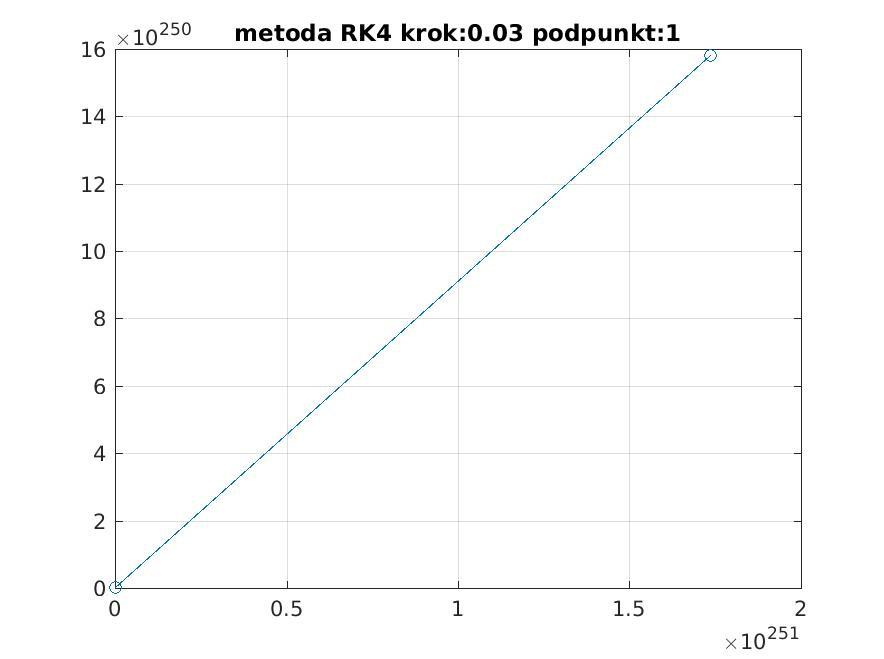
\includegraphics[width = 15cm]{2d/metoda RK4 krok:0,03 podpunkt:1.jpg}
\end{figure}

\begin{figure}[H]
\centering
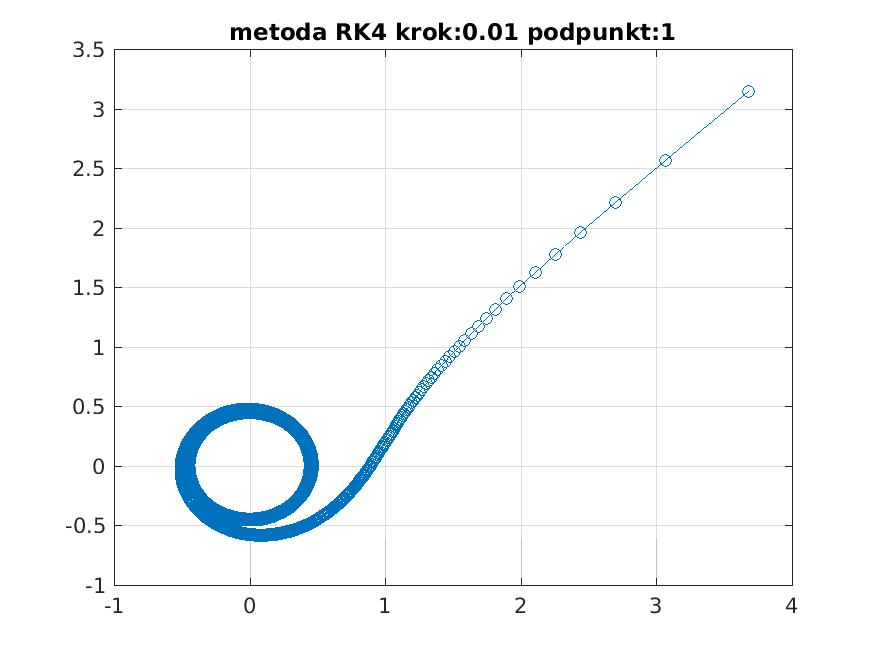
\includegraphics[width = 15cm]{2d/metoda RK4 krok:0,01 podpunkt:1.jpg}
\end{figure}

\begin{figure}[H]
\centering
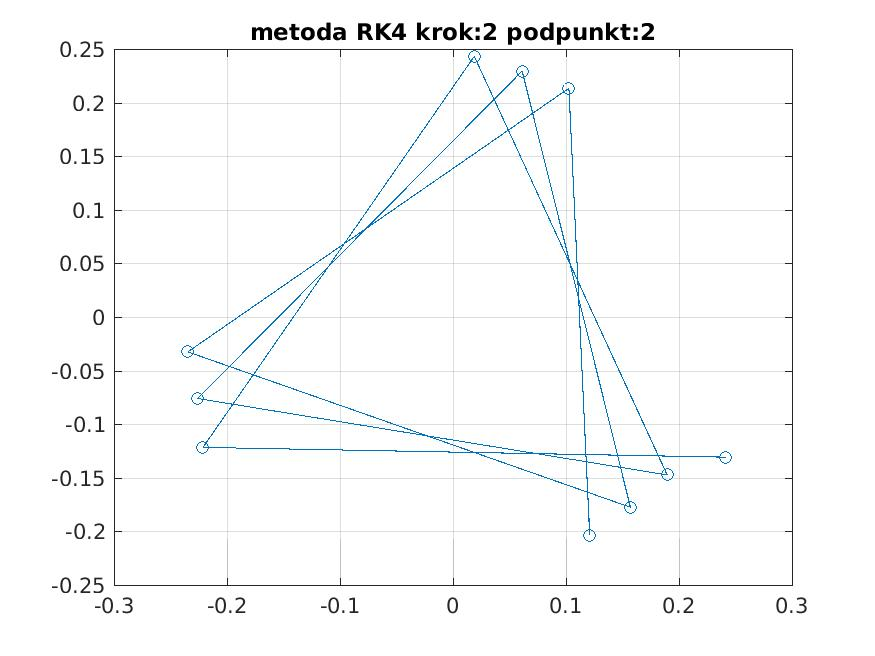
\includegraphics[width = 15cm]{2d/metoda RK4 krok:2 podpunkt:2.jpg}
\end{figure}

\begin{figure}[H]
\centering
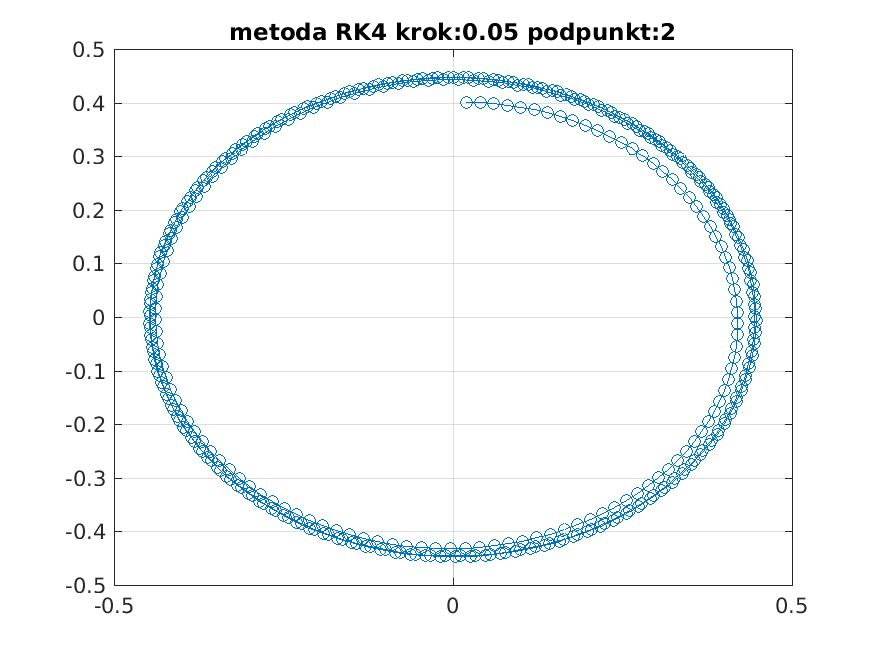
\includegraphics[width = 15cm]{2d/metoda RK4 krok:0,05 podpunkt:2.jpg}
\end{figure}

\begin{figure}[H]
\centering
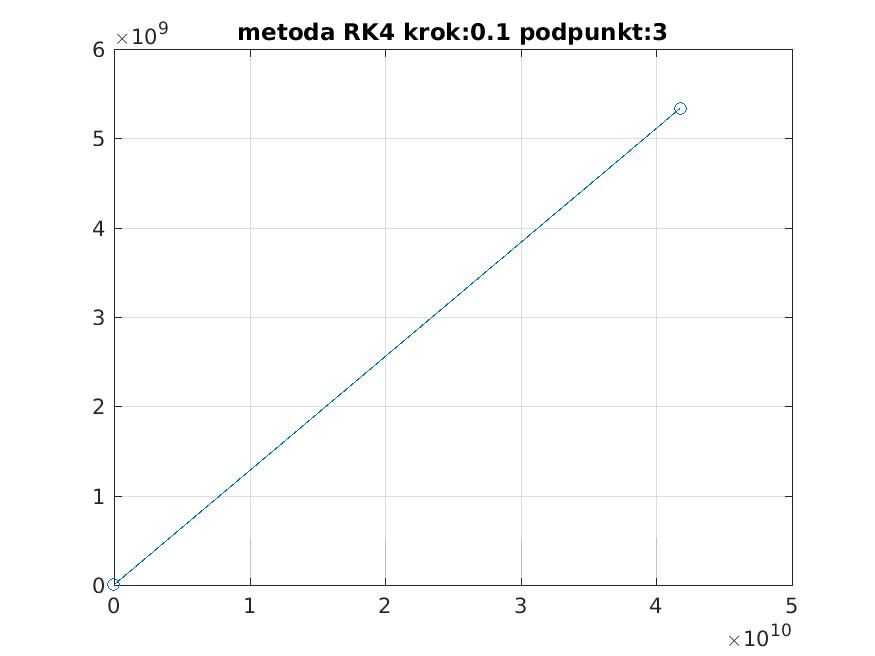
\includegraphics[width = 15cm]{2d/metoda RK4 krok:0,1 podpunkt:3.jpg}
\end{figure}

\begin{figure}[H]
\centering
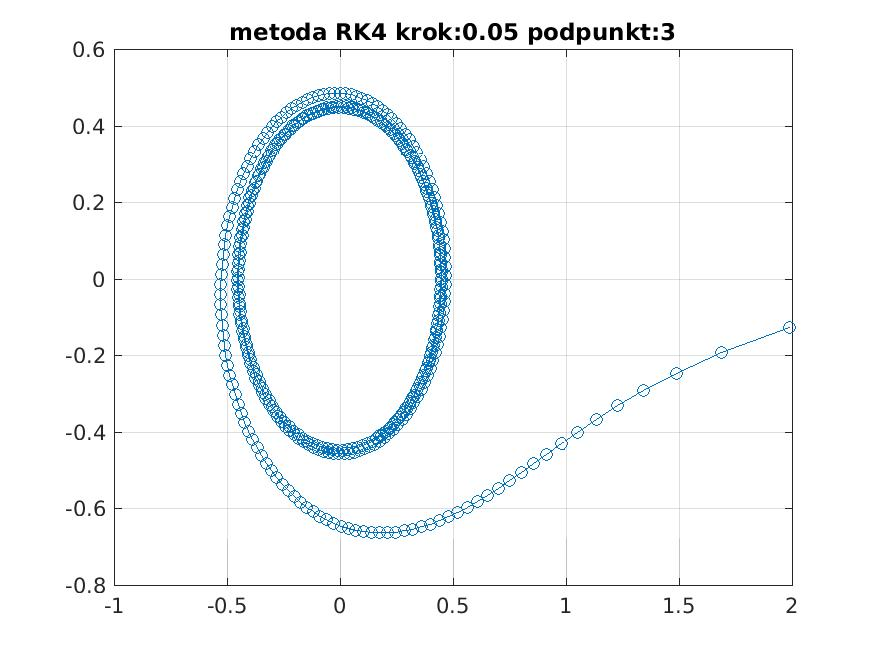
\includegraphics[width = 15cm]{2d/metoda RK4 krok:0,05 podpunkt:3.jpg}
\end{figure}

\begin{figure}[H]
\centering
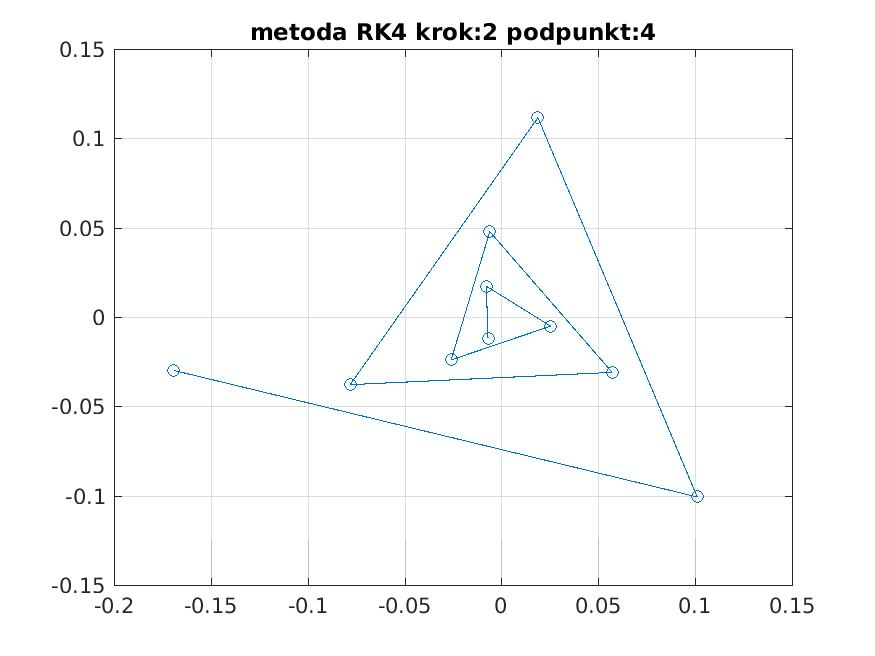
\includegraphics[width = 15cm]{2d/metoda RK4 krok:2 podpunkt:4.jpg}
\end{figure}

\begin{figure}[H]
\centering
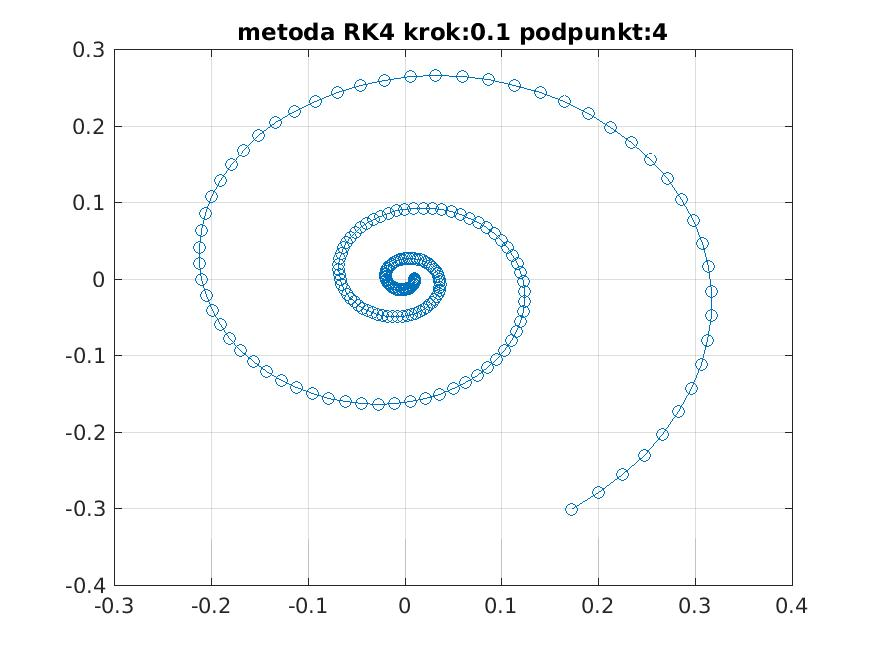
\includegraphics[width = 15cm]{2d/metoda RK4 krok:0,1 podpunkt:4.jpg}
\end{figure}

\subsection{Wnioski}
Metoda Rungego-Kutty dla podanych równań jest szybka przy odpowiednim kroku. Zmniejszając krok możaby coraz dokładniej wyznaczyć tor ruchu. Dobór odpowiedniej długości kroku w sposób interaktywny jest problematyczny ze względu na różnorodność kroków w zaleznosci od pountow startowych. Metoda róznież ma dość wysoki nakład obliczeniowy ponieważ jest on zależny tylko od przedziału i długości kroku, dlatego nie ma znaczenia czy równania są skomplikowane czy bardzo proste. 

\section{Metody wielokrokowe}
Metody wielokrokwe w odróżnieniu od iteracyjnych uzywają do wyznaczenia punktu wartości obliczonych w poprzednich krokach. Wynika z tego że przy rozpoczynaniu rozwiązywania zagadnienia metodą wielokrokową musimy wyznaczyć punkty początkowe (zazwiczaj jedną z metod iteracyjnych) a następnie na podstawie wartości początkowch obliczane są kolejne punkty. Medod tych używa się w przypadku gdy wyznaczanie wartości bezpośrednio ze wzoru jest czasochłonne, ponieważ metody wielokrokowe rzadziej wykorzystują bezpośrednie obliczanie wartości funkcji. Wyróżniamy metody jawne które wykorzystują jedynie wartości funkcji w poprzednio obliczonych punktach oraz niejawne, które dodatkowo korzystają z wartości w punkcie bierzącym. 

\subsection{Metoda predyktor-korektor Adamsa}
Metoda predykcyjno-korekcyjna łączy zalety metod jawnych i niejawnych. Dzięki temu zachowuje wysoki rząd i małą stałą błędu na szerokim obszarze przy zachowaniu małej liczby iteracji. Praktyczne realizacja metody polega na obliczeniu czterech członów: P - predykcja, E - ewaluacja, K - korekcja, E - kolejna ewaluacja. Dla metody predyktor - korektor Adamsa rozwiązanie możemy przybliżyć następującymi równaniami: 
$$P:  y_{n}^{[0]} = y_{n-1} + h \sum_{j=1}^{k} \beta_{j}f_{n-j}$$
$$E:  f_{n}^{[0]} = f(x_{n},y_{n}^{[0]})$$
$$K:  y_{n} = y_{n-1} + h \sum_{j=1}^{k} \beta_{j}^{*}f_{n-j}+h\beta_{0}^{*}f_{n}^{[0]}$$
$$E:  f_{n} = f(x_{n},y_{n})$$


\subsection{Realizacja funkcji RK4 w programie Matlab}
\begin{lstlisting}
function[Y] = md_pkadams(x,timelimit,stp)
%funkcja zwracajaca wektor wyznacziony metoda PK adamsa 
%dane wejsciowe
%x - wektor danych 
%timelimit - zakres czasu
%stp - dlugosc kroku
   
    Y = zeros(timelimit/stp,3); %wektor stanow x1, x2, czasu, i bledu
    hstp=stp/2;
    for i = 1:3 %generowanie punktow poczatkowych
        Y(i,3) = i*stp; %generowanie czasu
        k1 = md_fx(x); %pochodna w punkcie y(xn);
        k2 = md_fx(x+hstp*k1); %pochodna w punkcie y(xn+stp/2*k1) 
        k3 = md_fx(x+hstp*k2); %pochodna w punkcie y(xn+stp/2*k2)
        k4 = md_fx(x+stp*k3); %pochodna w punkcie y(xn+stp*k3)
        x=x+(1/6)*stp*(k1+2*k2+2*k3+k4); %obliczenie nastepnego punktu
        Y(i,1:2) = x; %zapisanie punktu do wektora
    end
    for i = 4:(timelimit/stp)
        Y(i,3) = i*stp; %gererowanie czasu
        tmp = x + stp/24*(55*md_fx(x) - 59*md_fx(Y(i-1,1:2)) + 37*md_fx(Y(i-2,1:2)) - 9*md_fx(Y(i-3,1:2))); % predykcja i ewaluacja
        x = x + stp/24*(9*md_fx(tmp) + 19*md_fx(x) - 5*md_fx(Y(i-1,1:2)) + md_fx(Y(i-2,1:2))); % korekcja i ewaluacja
        Y(i,1:2) = x; %zapis wyniku
    end
end

\end{lstlisting}


\subsection{Skrypt generujący wykresy do zadania}
\begin{lstlisting}
% Realizacja zadania 2 
% metoda metoda predyktor-korektor Adamsa 4-rzedu
clear; 
zero=[8 7; 0 0.4; 5 0; 0.01 0.001]; %wektor stanow poczatkowych
step = 0.01; %krok

for k = 1:1
    
    data = md_pkadams(zero(k,:),20,step);
   
    h = figure;%('visible','off');
    plot(data(:,1),data(:,2),'-o');
    l = size(data,1);
    hold on;
    grid on; 
    name =  ['metoda Adamsa krok:' num2str(step) ' podpunkt:' num2str(k)];
    title(name);
    saveas(h,name,'jpg'); 
end
\end{lstlisting}

\subsection{Dobieranie długości kroku}
Podobnie jak w poprzednim podpunkcie, długość kroku była wprowadzana przez użytkownika w trybie interaktywnym. 

\subsection{Wyniki}
\begin{figure}[H]
\centering
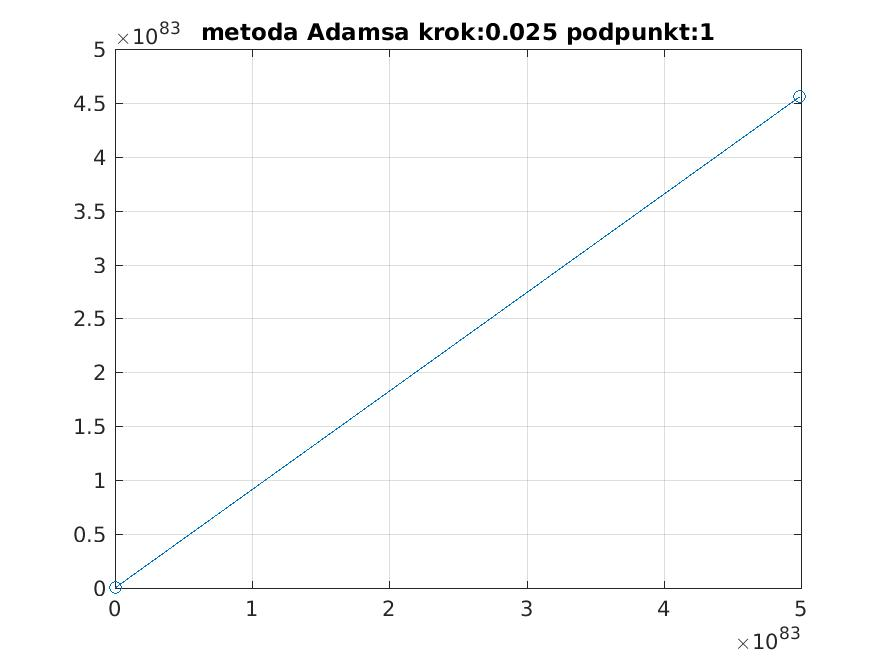
\includegraphics[width = 15cm]{2d/metoda Adamsa krok:0,025 podpunkt:1.jpg}
\end{figure}
\begin{figure}[H]
\centering
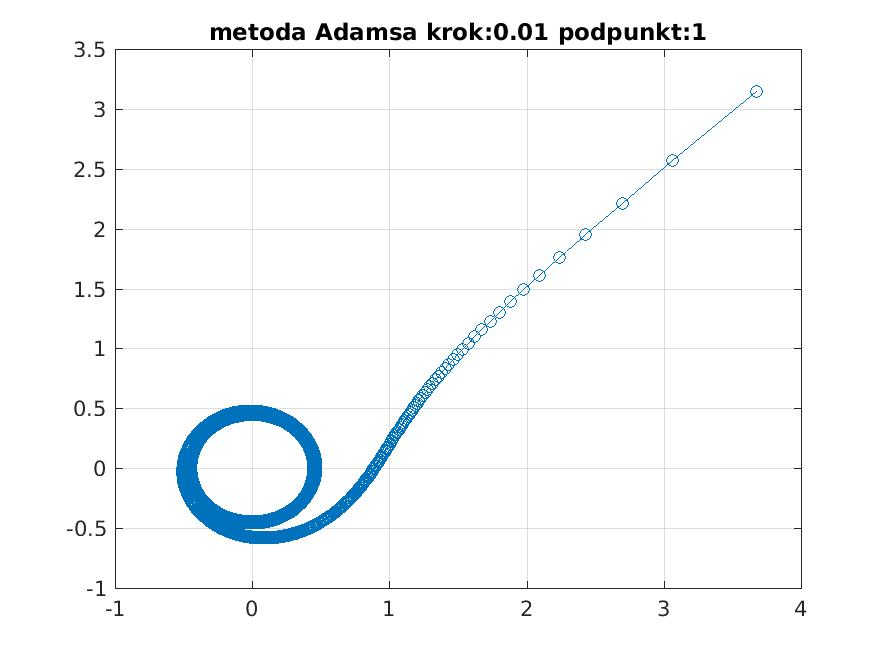
\includegraphics[width = 15cm]{2d/metoda Adamsa krok:0,01 podpunkt:1.jpg}
\end{figure}

\begin{figure}[H]
\centering
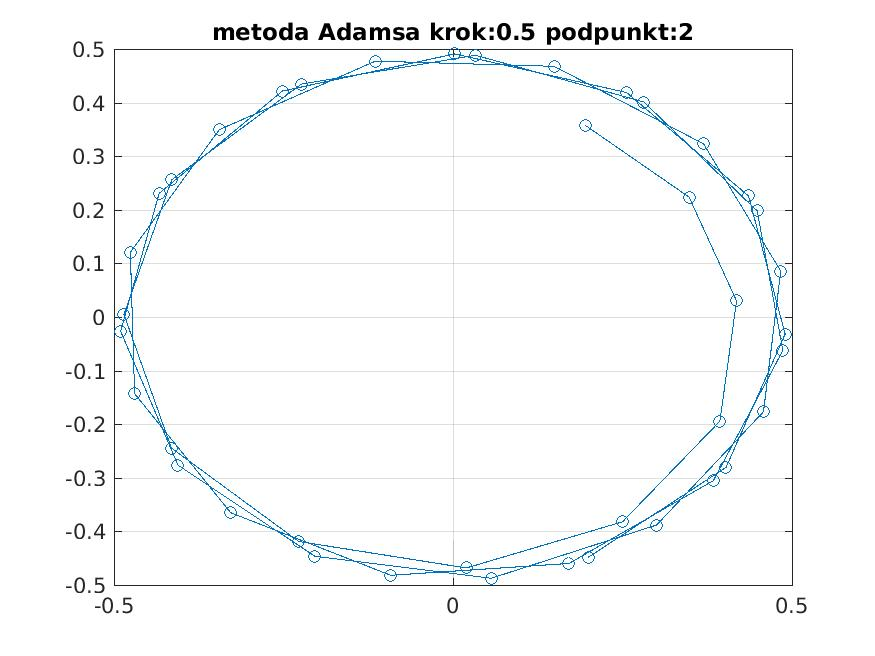
\includegraphics[width = 15cm]{2d/metoda Adamsa krok:0,5 podpunkt:2.jpg}
\end{figure}
\begin{figure}[H]
\centering
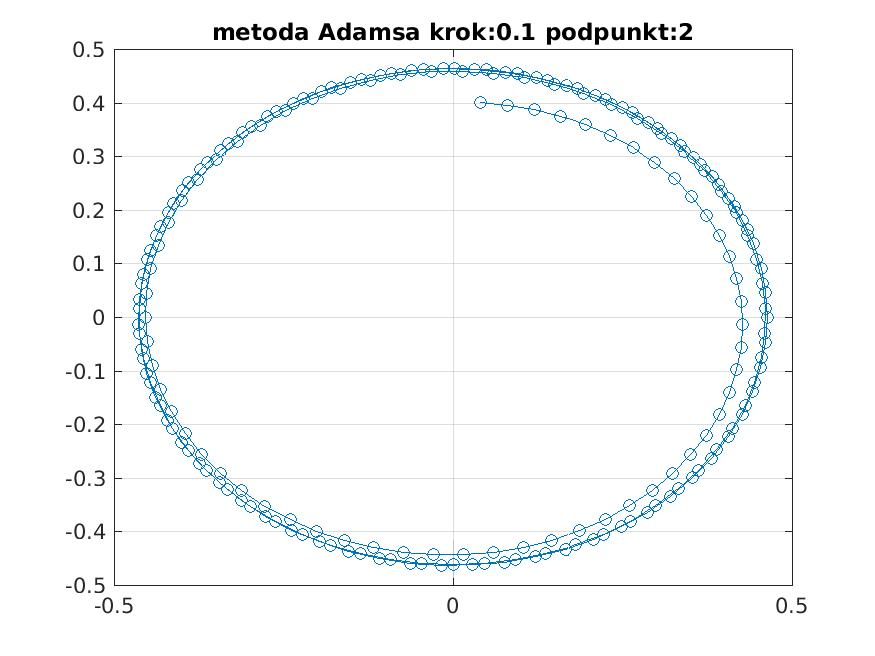
\includegraphics[width = 15cm]{2d/metoda Adamsa krok:0,1 podpunkt:2.jpg}
\end{figure}

\begin{figure}[H]
\centering
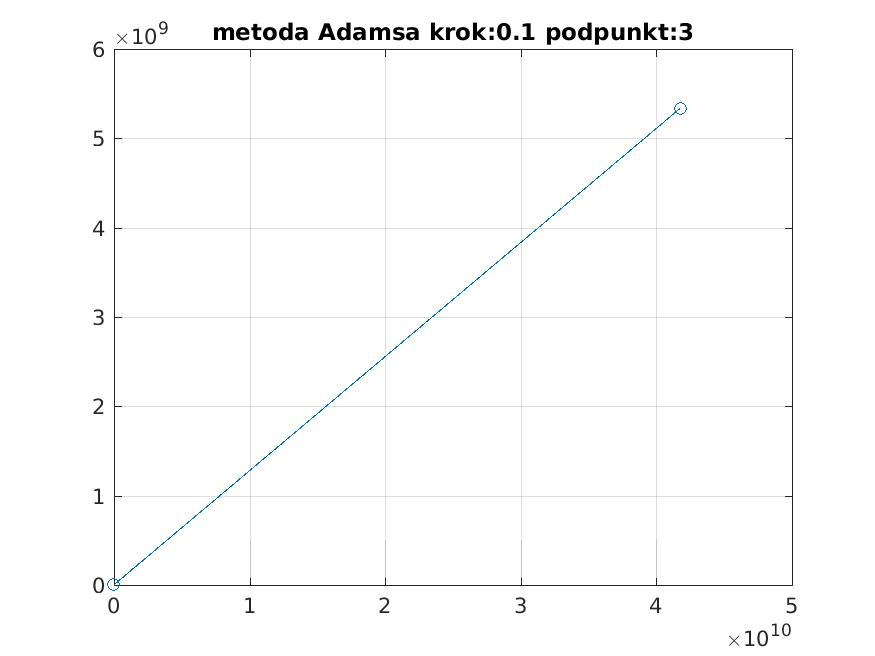
\includegraphics[width = 15cm]{2d/metoda Adamsa krok:0,1 podpunkt:3.jpg}
\end{figure}
\begin{figure}[H]
\centering
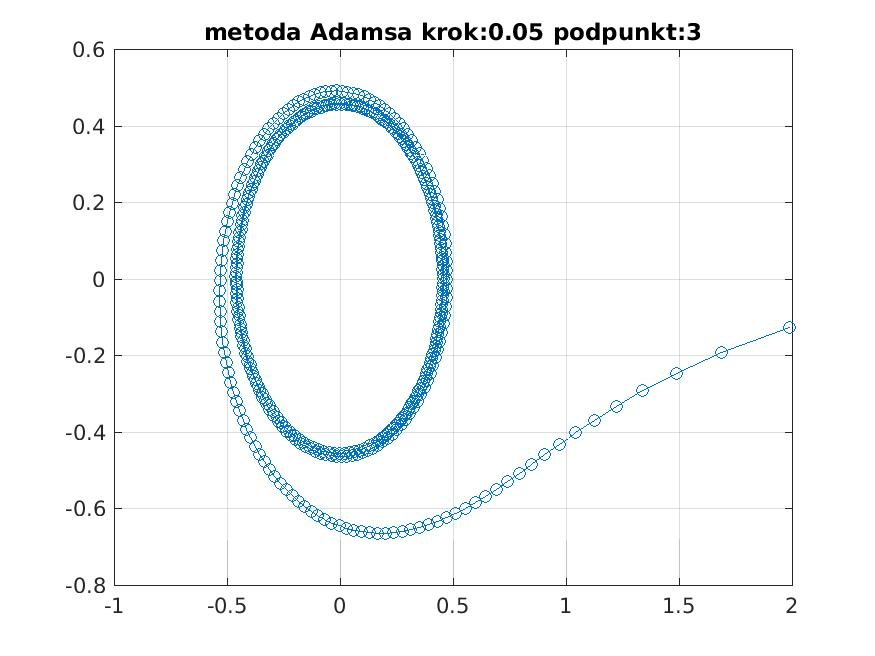
\includegraphics[width = 15cm]{2d/metoda Adamsa krok:0,05 podpunkt:3.jpg}
\end{figure}
\begin{figure}[H]
\centering
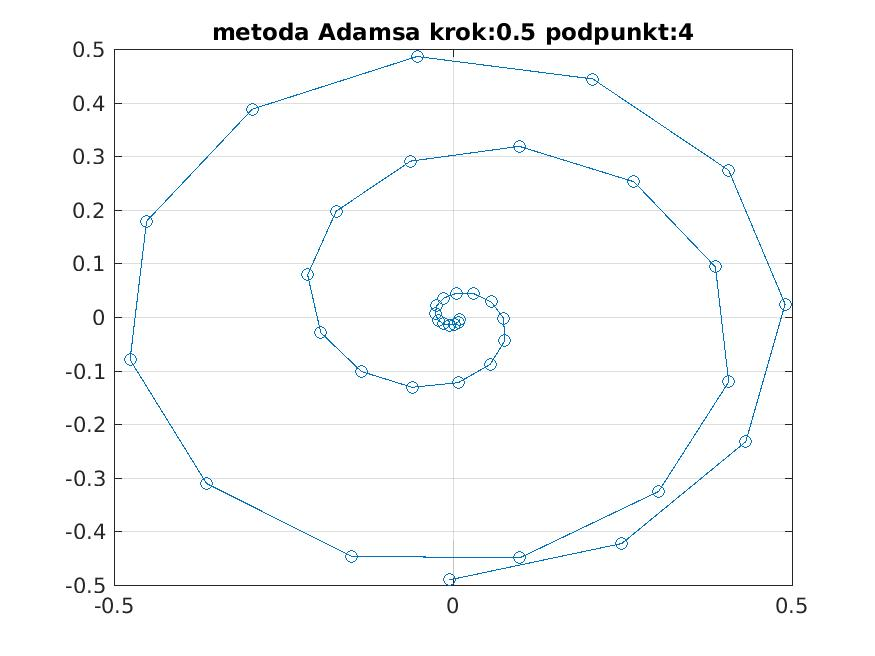
\includegraphics[width = 15cm]{2d/metoda Adamsa krok:0,5 podpunkt:4.jpg}
\end{figure}
\begin{figure}[H]
\centering
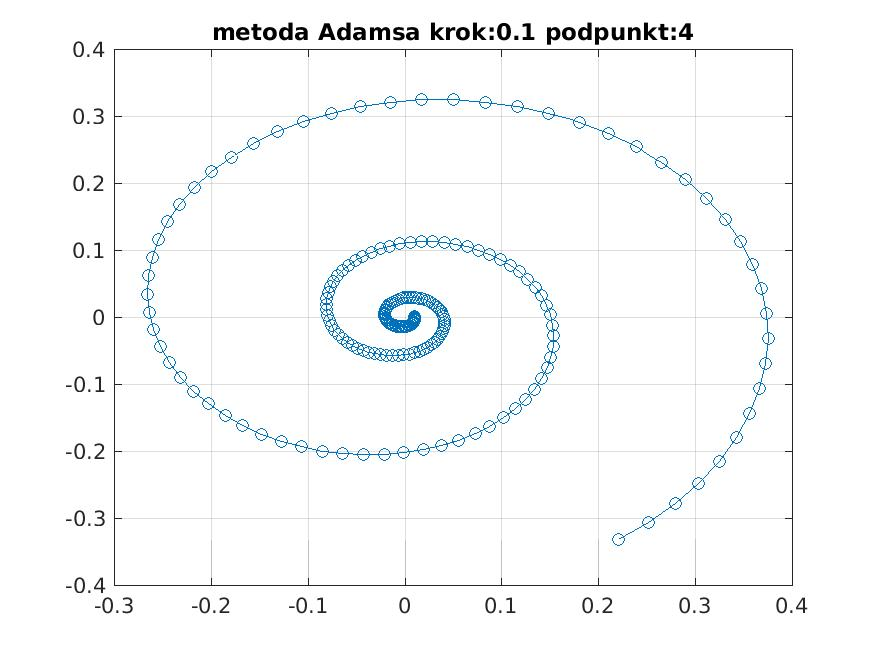
\includegraphics[width = 15cm]{2d/metoda Adamsa krok:0,1 podpunkt:4.jpg}
\end{figure}

\subsection{Wnioski}
Metoda predyktor-korektor Adamsa zdecydowanie dokładniej określa trajektorium niż metoda RK4 dla tego samego kroku, jednak potrzebuje znacznie mniejszego kroku do "ustabilizowania się". Różnica pomiędzy krokiem dla którego metoda jest zbieżna a krokiem dla którego jest dokłądna jest niewielka w przeciwieństwie do metody RK4. Dla dużych punktów początkowych metoda podobnie jak RK4 potrzebuje dosyć małego kroku aby uzyskać zbierzność na danym przedziale. 

\section{Metoda RK4 ze zmiennym krokiem}
\subsection{Opis algorytmu}
Jeżeli chodzi o metodę obliczeń to jest ona identyczna jak w tej ze stałym krokiem. Na szczególną uwagę zasługuje sposób oceny błędu i na tej podstawie regulacji długości kroku. Określanie błedu jest realizowane metodą połowienia kroku. W pojedyńczej iteracji obliczne są wartości funkcji dla całego kroku i jego połowy, następnie jeżeli różnica między otrzymanymi wartościami jest mniejsza niż założony współczynnik dokładności, to krok jest zwiększany, a gdy większa to zmniejszany. Jako wartość funkcji brana pod uwagę jest zawsze ta wyznaczona za pomocą dwóch mniejszych kroków. Długość kroku jest dodatkowo mnożona przez współczynnik bezpieczeństwa tak aby wzrost kroku nie był zbyt drastyczny, i aby również drastycznie nie zmalał, co doprowadziło by do znacznego wydłużenia czasu obliczeń. 

\subsection{Realizacja funkcji w programie Matlab}
\begin{lstlisting}
function [Y] = md_rk4d(x,timelimit,stp)
%RK4 Rozwiazanie ukladu metoda Rungego-Kutty czwartego rzedu ze zmiennym
%krokiem
%x - stan poczatkowy
%timelimit - zakres czasu
%step - rozmiar kroku

    
    Y=zeros(10,3);
    x1 = x;
    x2 = x;
    
    time = 0; %zmienna przechowujaca aktualny przedzial czasu
    i=1; %iterator indeksu wektorow

    while(time<=timelimit)
        
        k1 = md_fx(x1);
        k2 = md_fx(x1+(stp/2)*k1);
        k3 = md_fx(x1+(stp/2)*k2);
        k4 = md_fx(x1+stp*k3); 
        x1=x1+(1/6)*stp*(k1+2*k2+2*k3+k4);

        k1 = md_fx(x2);%obliczenie wartosci z polowicznym krokeim
        k2 = md_fx(x2+(stp/4)*k1);
        k3 = md_fx(x2+(stp/4)*k2);
        k4 = md_fx(x2+(stp/2)*k3);
        x2=x2+(1/6)*(stp/2)*(k1+2*k2+2*k3+k4);
        k1 = md_fx(x2);
        k2 = md_fx(x2+(stp/4)*k1);
        k3 = md_fx(x2+(stp/4)*k2);
        k4 = md_fx(x2+(stp/2)*k3);
        x2=x2+(1/6)*(stp/2)*(k1+2*k2+2*k3+k4);  
        
        R = (x2-x1)/15;
        
        if(abs(min(R))<0.00001) %kryterium bledu wzglednego  
            stp = stp*1.1;
        else
            if(stp>0.05)
                stp = stp*0.9;
            end
        end
        Y(i,1:2) = x2;
        time = time+stp; 
        disp(stp); 
        Y(i,3) = time; %zapisanie czasu
        i = i+1; 
    end
end

\end{lstlisting}

\subsection{Funkcja generująca rozwiązania do zadania}
\begin{lstlisting}
% Realizacja podpunktu 3 
% metoda metoda RK4 zmienny krok
clear; 
zero=[8 7; 0 0.4; 5 0; 0.01 0.001]; %wektor krokow
step = 0.01; %krok

for k = 1:4
    
    data = md_rk4d(zero(k,:),20,step);
    
    h = figure; %('visible','off')
    plot(data(:,1),data(:,2),'-o');
    l = size(data,1);
    hold on;
    grid on; 
    name =  ['metoda RK4 zmienny krok podpunkt:' num2str(k)];
    title(name);
    saveas(h,name,'jpg'); 
end
\end{lstlisting}
%
%\subsection{Wyniki}
%\begin{figure}[H]
%\centering
%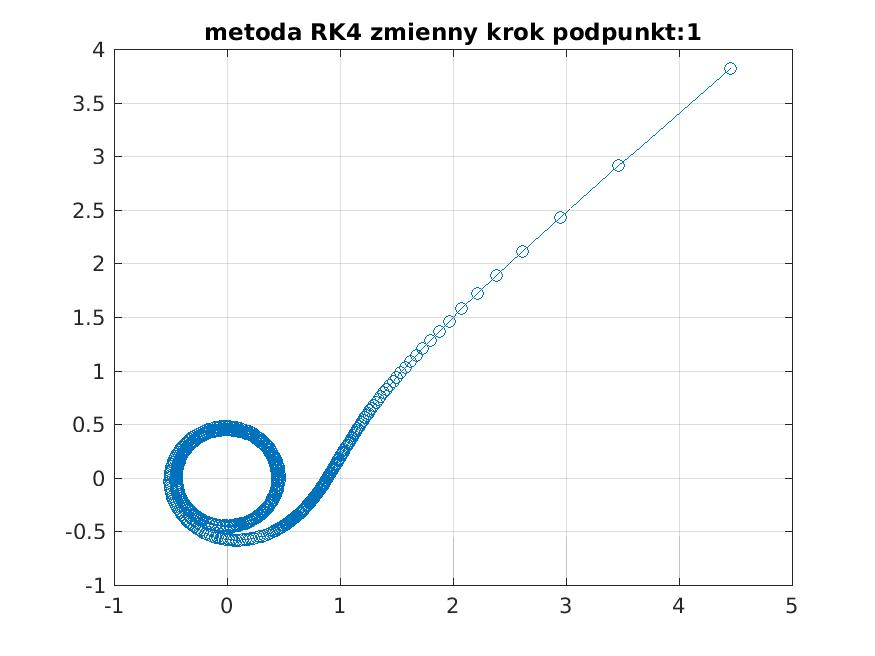
\includegraphics[width = 15cm]{2d/metoda RK4 zmienny krok podpunkt:1.jpg}
%\end{figure}
%\begin{figure}[H]
%\centering
%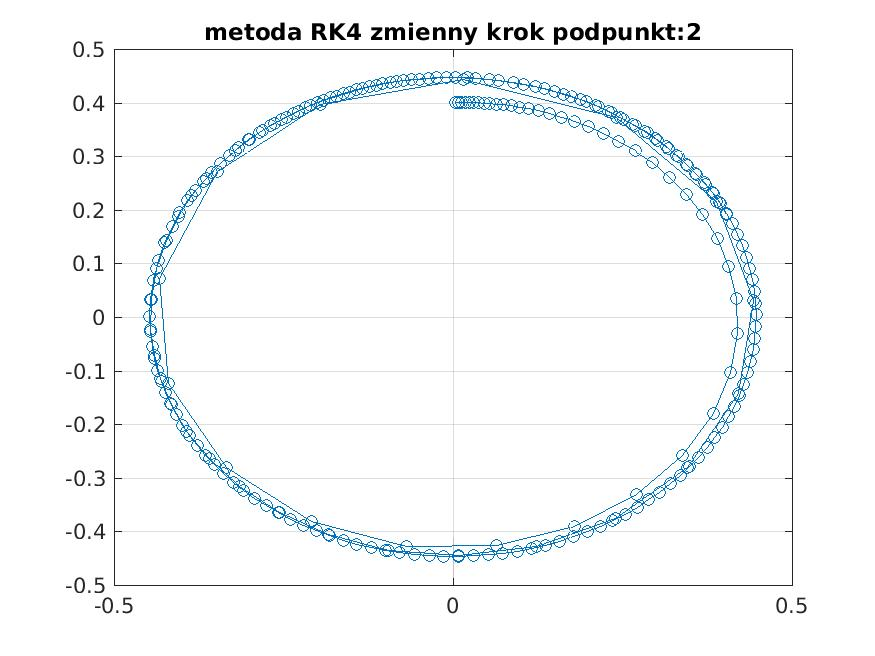
\includegraphics[width = 15cm]{2d/metoda RK4 zmienny krok podpunkt:2.jpg}
%\end{figure}
%\begin{figure}[H]
%\centering
%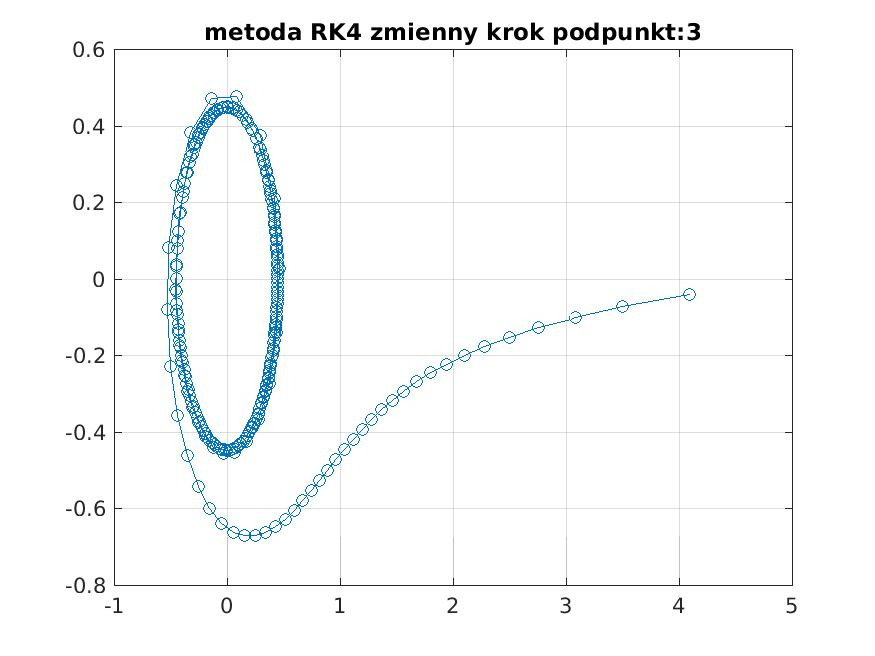
\includegraphics[width = 15cm]{2d/metoda RK4 zmienny krok podpunkt:3.jpg}
%\end{figure}
%\begin{figure}[H]
%\centering
%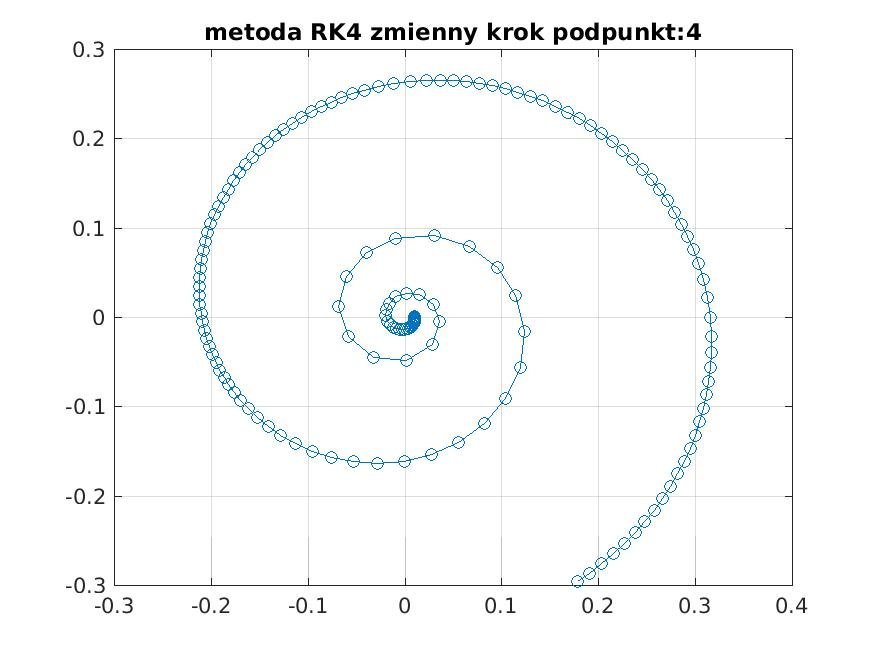
\includegraphics[width = 15cm]{2d/metoda RK4 zmienny krok podpunkt:4.jpg}
%\end{figure}

\subsection{Winoski}
Metoda RK4 ze zmiennym krokiem znacznie wydajniej radzi sobie z obliczeniami ze względu na istotne zmniejszenie liczby kroków na gładkich odcinkach funkcji. Zaimplementowana prze ze mnie megoda doboru długości kroku nie nalezy jednak do wyrafinowanych. Przez co wzrost wydajności nie jest szczególnie mocno zauważalny. 

\section{Porównanie z wynikami funkcji ode45}
Funkcja ode45 dobrała znacznie większe kroki co widać na wykresach, przez to czas obliczeń był rzędy razy mniejszy niż zaimplementowanych przeze mnie metod. Jeżeli chodzi o dokładność to wykresy wygenerowane funkcą ode45 są dużo mniej "gładkie" jednak krok jest dobierany równomiernie, i nie widać nakładjących się na siebie punktów na wykresie, co świadczy o optymalności metody. 

\begin{figure}[H]
\centering
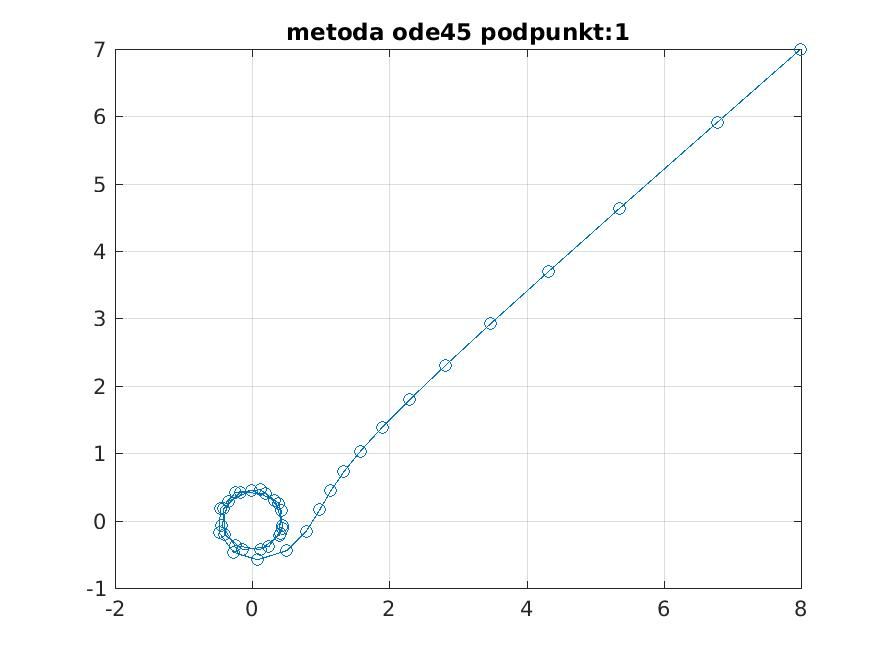
\includegraphics[width = 15cm]{ode/metoda ode45 podpunkt:1.jpg}
\end{figure}
\begin{figure}[H]
\centering
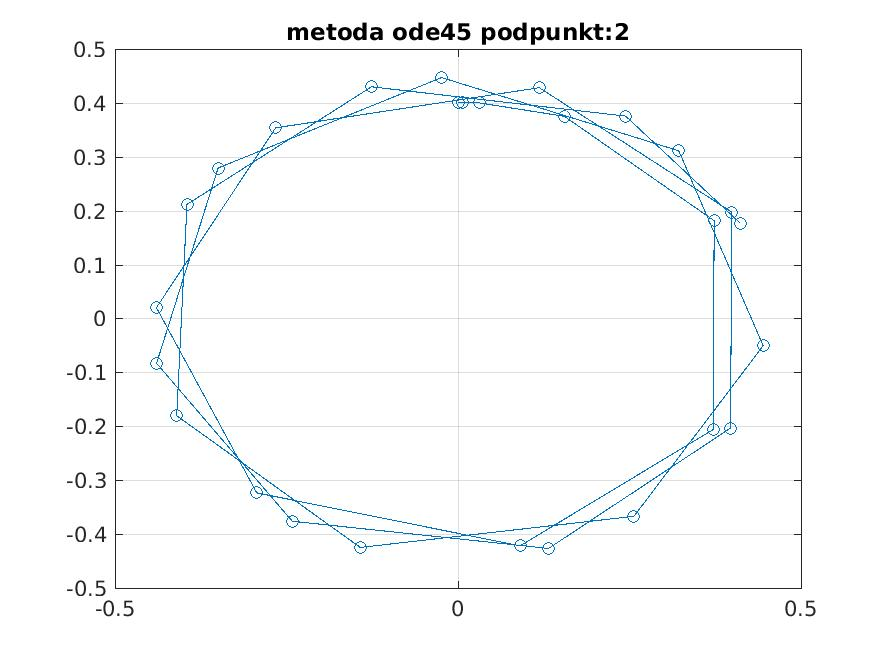
\includegraphics[width = 15cm]{ode/metoda ode45 podpunkt:2.jpg}
\end{figure}
\begin{figure}[H]
\centering
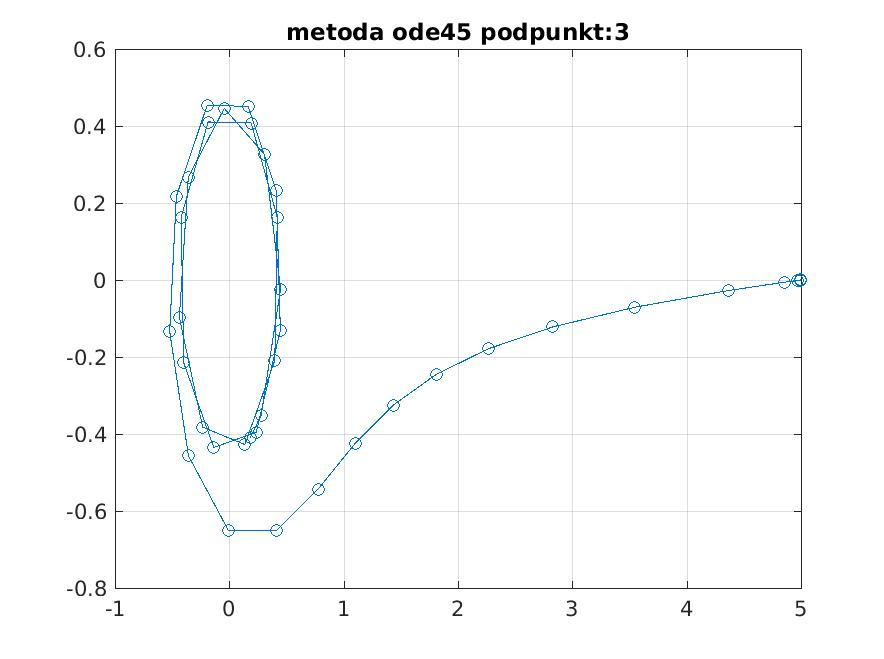
\includegraphics[width = 15cm]{ode/metoda ode45 podpunkt:3.jpg}
\end{figure}
\begin{figure}[H]
\centering
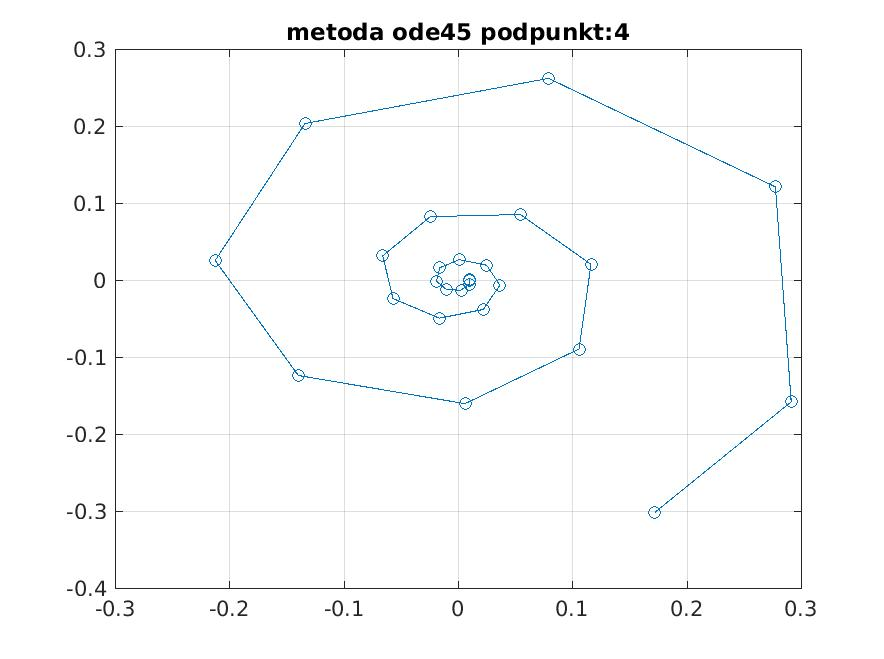
\includegraphics[width = 15cm]{ode/metoda ode45 podpunkt:4.jpg}
\end{figure}

\section{Wnioski końcowe}
W przypadku metod jednopunktowych stałokrokowych najlepiej wypada metoda adamsa ze względu na najniższy czas wykonania obliczeń, jednak jest ona zbierzna w wąskim przedziale kroku. Metoda RK4 ze zmiennym krokiem również bardzo dokładnie wyznacza trajektoriam jednak zdecydowanie przegrywa z metodą ode45 ze zmiennym krokiem pod względem wydajności. Przypuszczem że zastosowanie zmiennego kroku dla metody predyktor-korektor Adamsa mogło by dać najlepszy rezultat dla danych z tego zdania, ponieważ wymaga najmniejszej liczby kroków przy wysokiej dokładności. 


\end{document}


